\hypertarget{appendix-38d9c8aca357}{}
\section*{06 - Geometry and Vector Implementation - Visual Recall}
\chapter{From Movement to Meaning --- Geometry and Vector Implementation}\label{appendix-38d9c8aca357-from-movement-to-meaning-geometry-and-vector-implementation}

\textbf{Scope:} Companion to \href{Continuous\%20Notes/Computing\%20Foundations\%20-\%20From\%20Bits\%20to\%20C++\%20and\%20Systems\%20APIs\#The\%20panel\%20gives\%20us\%20a\%20reason\%20to\%20learn}{06 - From Movement to Meaning - Vectors, Geometry and Reliable Code}. The diagrams compress the robot-panel story; reconstruct the definitions, equations and failure cases from the chapter.

\section{One panel, one coordinate story}\label{appendix-38d9c8aca357-one-panel-one-coordinate-story}

\section{Four figure cards - read, hide, reconstruct}\label{appendix-38d9c8aca357-four-figure-cards---read-hide-reconstruct}

\begin{figure}
\centering
\pandocbounded{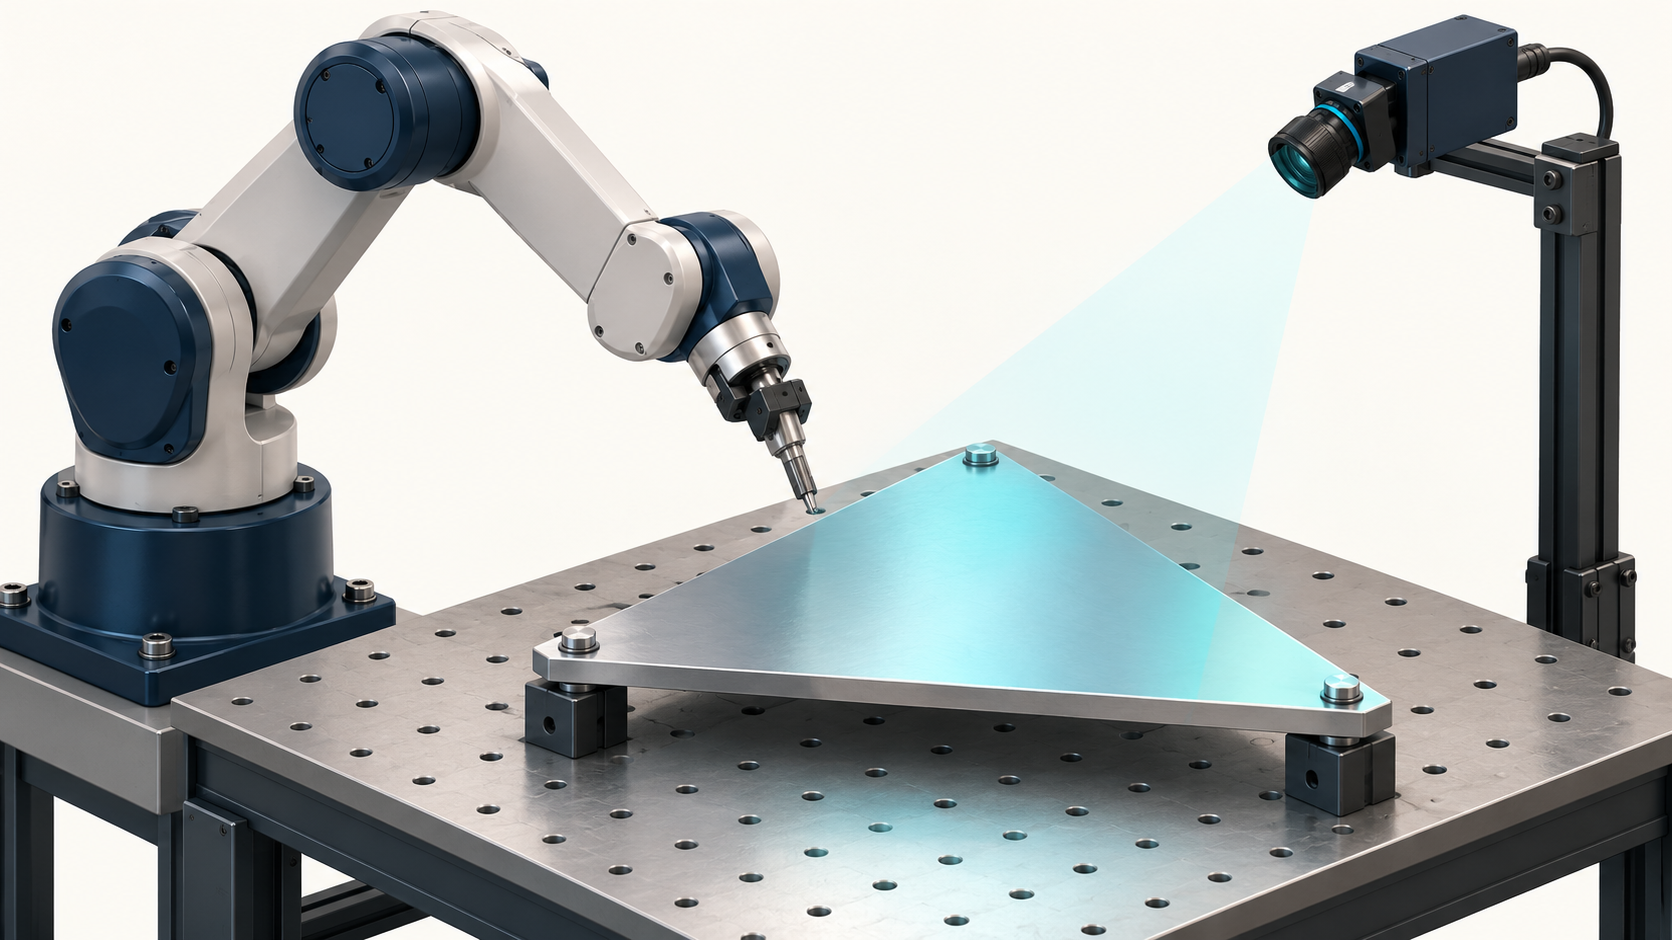
\includegraphics[keepaspectratio,alt={600}]{Visual Recall/geometry_robot_panel.png}}
\caption{600}
\end{figure}

\textbf{Scene cue:} identify the panel's corners, a sensor location, its displacement and a surface normal before writing components. The illustration is qualitative; its cyan cone is a schematic camera field of view. \href{Continuous\%20Notes/Computing\%20Foundations\%20-\%20From\%20Bits\%20to\%20C++\%20and\%20Systems\%20APIs\#Figure\%20G0\%20-\%20The\%20robot\%20and\%20its\%20inspection\%20panel}{Open Figure G0 and the numerical panel setup}.

Each card links to a captioned figure beside its full explanation in the continuous chapter. The numbers use the chapter's robot panel; each figure is compact and horizontal so it can be studied independently.

{\def\LTcaptype{none} % do not increment counter
\begin{longtable}[]{@{}
  >{\raggedright\arraybackslash}p{(\linewidth - 4\tabcolsep) * \real{0.3333}}
  >{\raggedright\arraybackslash}p{(\linewidth - 4\tabcolsep) * \real{0.3333}}
  >{\raggedright\arraybackslash}p{(\linewidth - 4\tabcolsep) * \real{0.3333}}@{}}
\toprule\noalign{}
\begin{minipage}[b]{\linewidth}\raggedright
Card
\end{minipage} & \begin{minipage}[b]{\linewidth}\raggedright
Shortest useful note
\end{minipage} & \begin{minipage}[b]{\linewidth}\raggedright
Figure and explanation
\end{minipage} \\
\midrule\noalign{}
\endhead
\bottomrule\noalign{}
\endlastfoot
\textbf{G1 · Role before tuple} & \(Q-P=\mathbf v\); \(P+\mathbf v=Q\). A basis changes components, not the arrow: \((3,2)=1(1,0)+2(1,1)\). A skew basis needs \(\|\mathbf v\|^2=c^\mathsf TGc=13\), not \(1^2+2^2\). & \href{Continuous\%20Notes/Computing\%20Foundations\%20-\%20From\%20Bits\%20to\%20C++\%20and\%20Systems\%20APIs\#G1\%20-\%20One\%20movement,\%20two\%20descriptions/}{Open Figure G1 and its limits} \\
\textbf{G2 · Along + across} & \(\mathbf p=\frac{\mathbf a\cdot\mathbf b}{\mathbf b\cdot\mathbf b}\mathbf b\); \(\mathbf r=\mathbf a-\mathbf p\). For \((3,4,0)\) along \((2,0,0)\): \(\alpha=1.5\), \(\mathbf p=(3,0,0)\), \(\mathbf r=(0,4,0)\). Require \(\mathbf b\ne0\); check \(\mathbf r\cdot\mathbf b=0\). & \href{Continuous\%20Notes/Computing\%20Foundations\%20-\%20From\%20Bits\%20to\%20C++\%20and\%20Systems\%20APIs\#G2\%20-\%20Split\%20the\%20request\%20into\%20rail\%20travel\%20and\%20sideways\%20travel/}{Open Figure G2 and the numerical trace} \\
\textbf{G3 · Location + interpolation} & \(P=\alpha A+\beta B+\gamma C\), \(\alpha+\beta+\gamma=1\). Panel weights \((5/12,1/4,1/3)\) give \(P=(1,1,0)\) and \(T=35\). Nonnegative weights mean inside only for an in-plane point and nondegenerate triangle. & \href{Continuous\%20Notes/Computing\%20Foundations\%20-\%20From\%20Bits\%20to\%20C++\%20and\%20Systems\%20APIs\#G3\%20-\%20Reconstruct\%20a\%20sensor\%20location\%20from\%20the\%20corners/}{Open Figure G3 and off-plane/perspective limits} \\
\textbf{G4 · Preserve perpendicularity} & \(\mathbf t'=A\mathbf t\), \(\mathbf n'=A^{-\mathsf T}\mathbf n\). For \(A=\operatorname{diag}(2,1,1)\), \((2,1,0)\cdot(1/2,-1,0)=0\). Check numerical usability; normalize shading normals after transformation. & \href{Continuous\%20Notes/Computing\%20Foundations\%20-\%20From\%20Bits\%20to\%20C++\%20and\%20Systems\%20APIs\#G4\%20-\%20Transform\%20the\%20normal\%20and\%20prove\%20the\%20relationship\%20survived/}{Open Figure G4 and failure branches} \\
\end{longtable}
}

\textbf{Recall test:} redraw one card without looking, reproduce its arithmetic, then state a case where its formula cannot safely be used. For uncertainty in determinant signs, reopen \href{Continuous\%20Notes/Computing\%20Foundations\%20-\%20From\%20Bits\%20to\%20C++\%20and\%20Systems\%20APIs\#A\%20predicate\%20needs\%20a\%20trustworthy\%20sign}{the predicate discussion} rather than adding a universal epsilon.

\subsection{Whole-story overview}\label{appendix-38d9c8aca357-whole-story-overview}

\pandocbounded{\includegraphics[keepaspectratio,alt={Diagram}]{/Users/swayamsingal/Library/Mobile Documents/iCloud~md~obsidian/Documents/Master/Book Production/AllMight Codex/QA/print-reference-dedup/assets/print/0d1f4f079c50ef6dfe9c7def3ada3b6fa87620b355ba336423ab8a177cda0788.pdf}}

\textbf{Caption:} Coordinates describe a geometric object relative to a basis; they are not the object itself. A point has a location role; a vector has a displacement role.

\section{Geometry operations by question}\label{appendix-38d9c8aca357-geometry-operations-by-question}

{\def\LTcaptype{none} % do not increment counter
\begin{longtable}[]{@{}
  >{\raggedright\arraybackslash}p{(\linewidth - 4\tabcolsep) * \real{0.3333}}
  >{\raggedright\arraybackslash}p{(\linewidth - 4\tabcolsep) * \real{0.3333}}
  >{\raggedright\arraybackslash}p{(\linewidth - 4\tabcolsep) * \real{0.3333}}@{}}
\toprule\noalign{}
\begin{minipage}[b]{\linewidth}\raggedright
Geometric question
\end{minipage} & \begin{minipage}[b]{\linewidth}\raggedright
Tool
\end{minipage} & \begin{minipage}[b]{\linewidth}\raggedright
Key interpretation / check
\end{minipage} \\
\midrule\noalign{}
\endhead
\bottomrule\noalign{}
\endlastfoot
How long is this displacement? & Norm & Scale inputs before squaring when range could overflow/underflow. \\
How aligned are two directions? & Dot product & Sign and magnitude depend on lengths; normalize only after validating nonzero finite inputs. \\
What part points along a direction? & Projection & Decompose into parallel and perpendicular components. \\
Which way is the oriented surface facing? & Cross product & Order/winding matters; magnitude is parallelogram area. \\
Which side or signed volume? & Determinant/triple product & Near-zero signs can be numerically uncertain. \\
Where inside the triangle? & Barycentric weights & Weights sum to one; perspective interpolation changes screen-space weights. \\
How do normals transform? & Inverse transpose & Preserve orthogonality to transformed tangents. \\
Are these shapes intersecting? & Convex support / Minkowski difference & Convert shared-point question to whether the origin is in the difference set. \\
\end{longtable}
}

\section{Coordinate frame: same movement, different coordinates}\label{appendix-38d9c8aca357-coordinate-frame-same-movement-different-coordinates}

\pandocbounded{\includegraphics[keepaspectratio,alt={Diagram}]{/Users/swayamsingal/Library/Mobile Documents/iCloud~md~obsidian/Documents/Master/Book Production/AllMight Codex/QA/print-reference-dedup/assets/print/e1ea4f19c2335e92e2c0d616d2e311cf9a49d9c6a91416955b6c94cd03f660f0.pdf}}

\textbf{Caption:} Changing components does not change the underlying vector. In a non-orthonormal basis, ordinary component dot products do not directly equal geometric inner products; the Gram matrix carries the metric.

\section{Robust computation: validate before normalizing or deciding}\label{appendix-38d9c8aca357-robust-computation-validate-before-normalizing-or-deciding}

\pandocbounded{\includegraphics[keepaspectratio,alt={Diagram}]{/Users/swayamsingal/Library/Mobile Documents/iCloud~md~obsidian/Documents/Master/Book Production/AllMight Codex/QA/print-reference-dedup/assets/print/c8c889d3471da0db99cba5f27389b5f457417f4fa3d03957393ca44888a76732.pdf}}

\textbf{Caption:} Clamping an invalid intermediate is not a proof that the original geometry was valid. Input validity, arithmetic range, tolerance meaning and decision confidence are separate checks.

\section{A three-number type is not the complete contract}\label{appendix-38d9c8aca357-a-three-number-type-is-not-the-complete-contract}

\begin{verbatim}
geometric promise  ──> initialization, role, units, space
storage promise    ──> size, alignment, offsets, stride
execution promise  ──> scalar/SIMD behavior and errors
boundary promise   ──> GPU format, shader layout, serialization
\end{verbatim}

\textbf{Caption:} A 12-byte CPU \texttt{Vec3} does not prove shader compatibility, array semantics, safe indexing, or a portable file representation.

\section{Retrieval prompts}\label{appendix-38d9c8aca357-retrieval-prompts}

\begin{enumerate}
\def\labelenumi{\arabic{enumi}.}
\tightlist
\item
  Why can point minus point produce a vector, but point plus point be meaningless?
\item
  What does a basis change alter, and what stays fixed?
\item
  Why does a cross-product sign depend on order and handedness?
\item
  Which exact conditions make a normalized vector meaningful?
\item
  Why does perspective correction change barycentric interpolation?
\item
  Why must the normal matrix be the inverse transpose?
\item
  What evidence distinguishes a robust predicate from a merely tested floating-point expression?
\end{enumerate}

\begin{quote}
{[}!answer{]}- Compact key Affine points have no intrinsic origin, while displacements do. Coordinates depend on the chosen basis; the geometric vector does not. Cross product is antisymmetric and encodes orientation. A direction needs finite, nonzero input and range-safe length computation. Perspective division is nonlinear, so interpolation must account for reciprocal depth. The inverse transpose preserves tangent-normal orthogonality under a general linear transform. A tested expression is evidence over those cases; a robust/certified claim requires stated assumptions and a procedure that guarantees the decision.
\end{quote}

\href{Continuous\%20Notes/Computing\%20Foundations\%20-\%20From\%20Bits\%20to\%20C++\%20and\%20Systems\%20APIs\#The\%20panel\%20gives\%20us\%20a\%20reason\%20to\%20learn}{Teach the full Phase 6 story} · \href{../01-Foundations-I/main.pdf\#nameddest=appendix-fd090d982a15-phase-6---parts-501-600}{Part coverage (01-Foundations-I, appendix-fd090d982a15-phase-6-\/-\/-parts-501-600)} · \href{Continuous\%20Notes/Computing\%20Foundations\%20-\%20From\%20Bits\%20to\%20C++\%20and\%20Systems\%20APIs\#Phase\%206\%20-\%20Geometry\%20reconstruction\%20proofs}{Derivations}

\section{One-page active-recall mini-atlas}\label{appendix-38d9c8aca357-one-page-active-recall-mini-atlas}

Use each row as a prompt: say the rule, state its precondition, then point to the linked chapter section for the full explanation and figures. The short cues are retrieval hooks, not replacements for the teaching narrative.

{\def\LTcaptype{none} % do not increment counter
\begin{longtable}[]{@{}
  >{\raggedright\arraybackslash}p{(\linewidth - 4\tabcolsep) * \real{0.3333}}
  >{\raggedright\arraybackslash}p{(\linewidth - 4\tabcolsep) * \real{0.3333}}
  >{\raggedright\arraybackslash}p{(\linewidth - 4\tabcolsep) * \real{0.3333}}@{}}
\toprule\noalign{}
\begin{minipage}[b]{\linewidth}\raggedright
Recall cue
\end{minipage} & \begin{minipage}[b]{\linewidth}\raggedright
Shortest useful note
\end{minipage} & \begin{minipage}[b]{\linewidth}\raggedright
Reopen in the continuous chapter
\end{minipage} \\
\midrule\noalign{}
\endhead
\bottomrule\noalign{}
\endlastfoot
\textbf{What is the robot trying to represent?} & A tuple is only storage; decide whether it means a point, displacement, direction, unit normal, or measurement, and state its frame and units. & \href{Continuous\%20Notes/Computing\%20Foundations\%20-\%20From\%20Bits\%20to\%20C++\%20and\%20Systems\%20APIs\#The\%20panel\%20gives\%20us\%20a\%20reason\%20to\%20learn/}{Panel and problem setup} · \href{Continuous\%20Notes/Computing\%20Foundations\%20-\%20From\%20Bits\%20to\%20C++\%20and\%20Systems\%20APIs\#Three\%20stored\%20numbers\%20are\%20not\%20the\%20complete\%20contract/}{Vec3 contracts} \\
\textbf{What changes when I change coordinates?} & The geometric vector stays fixed; its components change with the basis. A skew basis needs its Gram matrix to measure angles and lengths correctly. & \href{Continuous\%20Notes/Computing\%20Foundations\%20-\%20From\%20Bits\%20to\%20C++\%20and\%20Systems\%20APIs\#An\%20arrow\%20is\%20not\%20the\%20address\%20written\%20beside\%20it/}{Points and vectors} · \href{Continuous\%20Notes/Computing\%20Foundations\%20-\%20From\%20Bits\%20to\%20C++\%20and\%20Systems\%20APIs\#A\%20basis\%20is\%20a\%20measuring\%20arrangement,\%20not\%20the\%20vector\%20itself/}{Basis change} · \href{Continuous\%20Notes/Computing\%20Foundations\%20-\%20From\%20Bits\%20to\%20C++\%20and\%20Systems\%20APIs\#A\%20Gram\%20matrix\%20remembers\%20the\%20geometry\%20of\%20a\%20slanted\%20basis/}{Gram matrix} \\
\textbf{Can the robot reach this movement?} & Allowed combinations form a span; closure under addition and scalar scaling makes a subspace. Independence means no control direction is redundant. & \href{Continuous\%20Notes/Computing\%20Foundations\%20-\%20From\%20Bits\%20to\%20C++\%20and\%20Systems\%20APIs\#The\%20reachable\%20movements\%20form\%20a\%20vector\%20space/}{Reachability and independence} \\
\textbf{How much, which way, how aligned?} & Norm measures length; dot measures alignment; projection extracts a component. Check finite/nonzero inputs before normalization and scale before squaring. & \href{Continuous\%20Notes/Computing\%20Foundations\%20-\%20From\%20Bits\%20to\%20C++\%20and\%20Systems\%20APIs\#A\%20ruler\%20needs\%20more\%20than\%20coordinate\%20components/}{Norm and distance} · \href{Continuous\%20Notes/Computing\%20Foundations\%20-\%20From\%20Bits\%20to\%20C++\%20and\%20Systems\%20APIs\#The\%20dot\%20product\%20turns\%20two\%20movements\%20into\%20a\%20measurement/}{Dot and angle} · \href{Continuous\%20Notes/Computing\%20Foundations\%20-\%20From\%20Bits\%20to\%20C++\%20and\%20Systems\%20APIs\#Projection\%20separates\%20useful\%20movement\%20from\%20sideways\%20movement/}{Projection} \\
\textbf{Which side is the panel facing?} & Cross-product order encodes orientation; magnitude is area. A triple product gives signed volume; near-zero signs need a reliability policy. & \href{Continuous\%20Notes/Computing\%20Foundations\%20-\%20From\%20Bits\%20to\%20C++\%20and\%20Systems\%20APIs\#Oriented\%20area\%20tells\%20us\%20which\%20side\%20of\%20the\%20panel\%20is\%20front/}{Cross product and winding} · \href{Continuous\%20Notes/Computing\%20Foundations\%20-\%20From\%20Bits\%20to\%20C++\%20and\%20Systems\%20APIs\#Signed\%20volume\%20extends\%20the\%20same\%20idea\%20into\%20space/}{Signed volume} \\
\textbf{How do I make a stable local surface frame?} & Choose tangents, reject the unwanted component, then normalize safely. Gram--Schmidt is repeated rejection; order and precision affect the result. & \href{Continuous\%20Notes/Computing\%20Foundations\%20-\%20From\%20Bits\%20to\%20C++\%20and\%20Systems\%20APIs\#Surface\%20movement\%20becomes\%20a\%20local\%20frame/}{Surface frame} · \href{Continuous\%20Notes/Computing\%20Foundations\%20-\%20From\%20Bits\%20to\%20C++\%20and\%20Systems\%20APIs\#Orthonormal\%20frames\%20make\%20reconstruction\%20simple/}{Orthonormal frame} \\
\textbf{How does geometry become shading?} & Reflection flips the normal component; refraction changes the tangent component. Normals are covectors: transform them with inverse transpose to preserve perpendicularity. & \href{Continuous\%20Notes/Computing\%20Foundations\%20-\%20From\%20Bits\%20to\%20C++\%20and\%20Systems\%20APIs\#Light\%20uses\%20the\%20same\%20decomposition\%20in\%20a\%20new\%20role/}{Lighting decomposition} · \href{Continuous\%20Notes/Computing\%20Foundations\%20-\%20From\%20Bits\%20to\%20C++\%20and\%20Systems\%20APIs\#A\%20normal\%20is\%20a\%20measuring\%20rule\%20before\%20it\%20is\%20an\%20arrow/}{Normal transform} \\
\textbf{Where is the sensor on the triangle?} & Barycentric weights sum to one; they locate points and interpolate attributes. Perspective projection changes screen-space weights; orientation predicates need trustworthy signs. & \href{Continuous\%20Notes/Computing\%20Foundations\%20-\%20From\%20Bits\%20to\%20C++\%20and\%20Systems\%20APIs\#The\%20sensor\%20needs\%20coordinates\%20inside\%20the\%20triangle/}{Barycentric coordinates and predicates} \\
\textbf{When do shapes touch?} & Convex combinations describe convex shapes; a Minkowski difference turns intersection into asking whether the origin belongs to the difference. & \href{Continuous\%20Notes/Computing\%20Foundations\%20-\%20From\%20Bits\%20to\%20C++\%20and\%20Systems\%20APIs\#Weighted\%20points\%20lead\%20from\%20affine\%20geometry\%20to\%20collision\%20shapes/}{Convexity and collision} \\
\textbf{Why add a fourth coordinate?} & Homogeneous coordinates let matrix operations express translation; projective points have equivalent scaled representatives. NDC is not a normalized direction. & \href{Continuous\%20Notes/Computing\%20Foundations\%20-\%20From\%20Bits\%20to\%20C++\%20and\%20Systems\%20APIs\#Homogeneous\%20coordinates\%20preserve\%20the\%20role\%20of\%20a\%20location/}{Homogeneous and projective coordinates} \\
\textbf{What can the computer invalidate?} & Floating-point arithmetic can overflow, underflow, lose small changes, or give an uncertain sign. Validate inputs, scale safely, then apply explicit tolerance/error policy. & \href{Continuous\%20Notes/Computing\%20Foundations\%20-\%20From\%20Bits\%20to\%20C++\%20and\%20Systems\%20APIs\#The\%20machine\%20is\%20a\%20model\%20of\%20the\%20field,\%20not\%20the\%20field/}{Floating-point model} · \href{Continuous\%20Notes/Computing\%20Foundations\%20-\%20From\%20Bits\%20to\%20C++\%20and\%20Systems\%20APIs\#Reliability\%20begins\%20at\%20the\%20boundary\%20of\%20the\%20calculation/}{Numerical boundary} \\
\textbf{What must the C++ type/API promise?} & Separate geometric role, units, scalar precision, memory layout, SIMD behavior, and GPU/serialization agreement; \texttt{Vec3} alone proves none of the external contracts. & \href{Continuous\%20Notes/Computing\%20Foundations\%20-\%20From\%20Bits\%20to\%20C++\%20and\%20Systems\%20APIs\#Types\%20can\%20remember\%20the\%20promises\%20that\%20three\%20components\%20forget/}{Semantic types} · \href{Continuous\%20Notes/Computing\%20Foundations\%20-\%20From\%20Bits\%20to\%20C++\%20and\%20Systems\%20APIs\#Storage\%20and\%20computation\%20can\%20choose\%20different\%20layouts/}{CPU/GPU layout} · \href{Continuous\%20Notes/Computing\%20Foundations\%20-\%20From\%20Bits\%20to\%20C++\%20and\%20Systems\%20APIs\#A\%20complete\%20scalar\%20laboratory\%20makes\%20the\%20story\%20executable/}{Executable reference and tests} \\
\end{longtable}
}

\section{Landscape concept maps}\label{appendix-38d9c8aca357-landscape-concept-maps}

\subsection{The panel: from geometry to engine data}\label{appendix-38d9c8aca357-the-panel-from-geometry-to-engine-data}

\pandocbounded{\includegraphics[keepaspectratio,alt={Diagram}]{/Users/swayamsingal/Library/Mobile Documents/iCloud~md~obsidian/Documents/Master/Book Production/AllMight Codex/QA/print-reference-dedup/assets/print/73eb308dd80a200a1584c875887fba550ae6a01f515a94015bd0b01b7ff1c8c1.pdf}}

\textbf{Caption:} Read left to right as the robot's work, not a list of disconnected formulas. Revisit \href{Continuous\%20Notes/Computing\%20Foundations\%20-\%20From\%20Bits\%20to\%20C++\%20and\%20Systems\%20APIs\#The\%20panel\%20gives\%20us\%20a\%20reason\%20to\%20learn}{the panel setup} and \href{Continuous\%20Notes/Computing\%20Foundations\%20-\%20From\%20Bits\%20to\%20C++\%20and\%20Systems\%20APIs\#The\%20sensor\%20needs\%20coordinates\%20inside\%20the\%20triangle}{the sensor\textquotesingle s triangle coordinates}.

\subsection{Three tools, three different questions}\label{appendix-38d9c8aca357-three-tools-three-different-questions}

\pandocbounded{\includegraphics[keepaspectratio,alt={Diagram}]{/Users/swayamsingal/Library/Mobile Documents/iCloud~md~obsidian/Documents/Master/Book Production/AllMight Codex/QA/print-reference-dedup/assets/print/c4e8f60d9c68fecb7a78e10fcaaa649b62f12220d503dda1e5213c58892b1111.pdf}}

\textbf{Caption:} Do not substitute one operation for another: they answer different geometric questions. See \href{Continuous\%20Notes/Computing\%20Foundations\%20-\%20From\%20Bits\%20to\%20C++\%20and\%20Systems\%20APIs\#The\%20dot\%20product\%20turns\%20two\%20movements\%20into\%20a\%20measurement}{dot}, \href{Continuous\%20Notes/Computing\%20Foundations\%20-\%20From\%20Bits\%20to\%20C++\%20and\%20Systems\%20APIs\#Oriented\%20area\%20tells\%20us\%20which\%20side\%20of\%20the\%20panel\%20is\%20front}{cross}, and \href{Continuous\%20Notes/Computing\%20Foundations\%20-\%20From\%20Bits\%20to\%20C++\%20and\%20Systems\%20APIs\#Projection\%20separates\%20useful\%20movement\%20from\%20sideways\%20movement}{projection}.

\subsection{Reliability ladder}\label{appendix-38d9c8aca357-reliability-ladder}

\pandocbounded{\includegraphics[keepaspectratio,alt={Diagram}]{/Users/swayamsingal/Library/Mobile Documents/iCloud~md~obsidian/Documents/Master/Book Production/AllMight Codex/QA/print-reference-dedup/assets/print/d9a3e10d3b019159339497a1c80b27b8bcc0f909f7e1e1250a53201887d4f2b1.pdf}}

\textbf{Caption:} A mathematically valid construction is not automatically a reliable machine decision. Follow \href{Continuous\%20Notes/Computing\%20Foundations\%20-\%20From\%20Bits\%20to\%20C++\%20and\%20Systems\%20APIs\#A\%20direction\%20can\%20exist\%20even\%20when\%20the\%20naive\%20length\%20overflows}{safe norm}, \href{Continuous\%20Notes/Computing\%20Foundations\%20-\%20From\%20Bits\%20to\%20C++\%20and\%20Systems\%20APIs\#A\%20predicate\%20needs\%20a\%20trustworthy\%20sign}{predicate reliability}, and \href{Continuous\%20Notes/Computing\%20Foundations\%20-\%20From\%20Bits\%20to\%20C++\%20and\%20Systems\%20APIs\#Reliability\%20begins\%20at\%20the\%20boundary\%20of\%20the\%20calculation}{calculation boundary}.

\section{Added retrieval prompt}\label{appendix-38d9c8aca357-added-retrieval-prompt}

Camera framing uses a point angle atan2(y,z); double the largest half-angle for full vertical FOV; include asin(r/d) for a sphere. \href{Continuous\%20Notes/Computing\%20Foundations\%20-\%20From\%20Bits\%20to\%20C++\%20and\%20Systems\%20APIs\#Projection\%20separates\%20useful\%20movement\%20from\%20sideways\%20movement}{Rebuild the camera trace}.

\begin{figure}
\centering
\pandocbounded{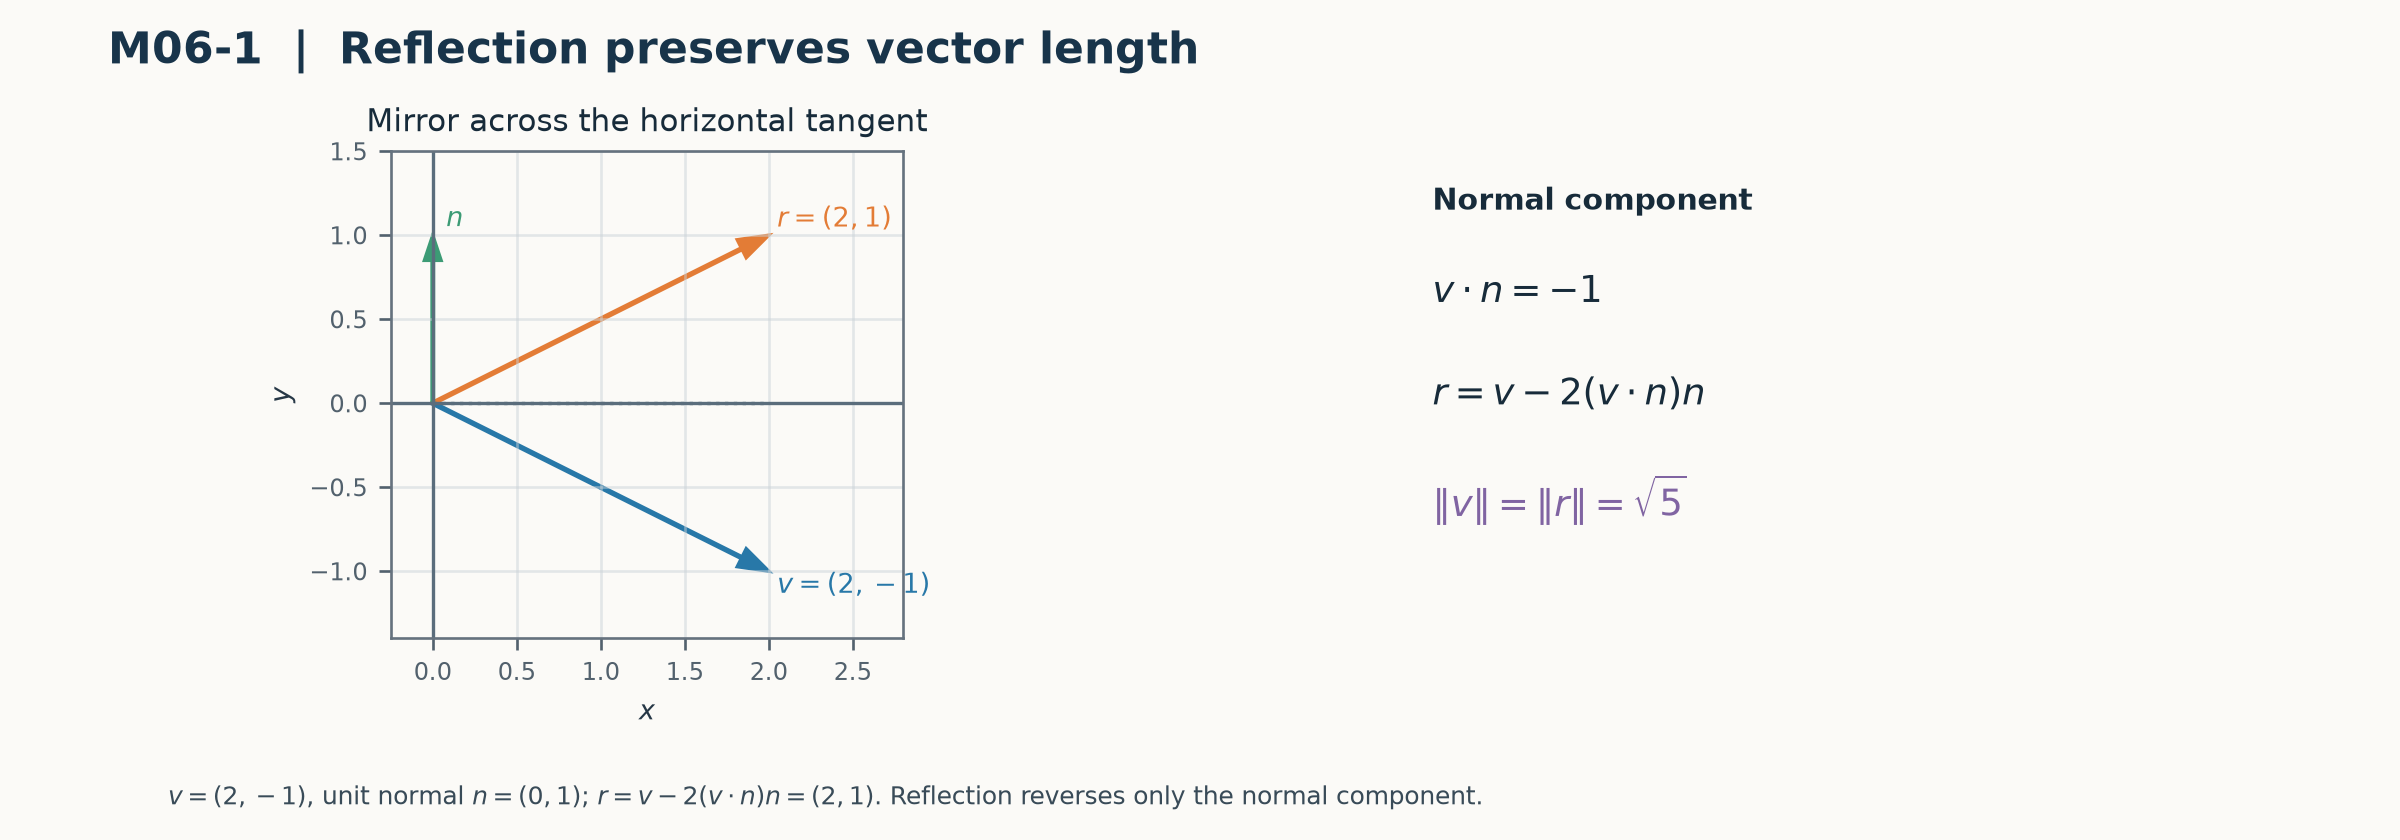
\includegraphics[keepaspectratio,alt={Visual Recall/Math Foundations/M06-1\_vector-reflection.png}]{Visual Recall/Math Foundations/M06-1_vector-reflection.png}}
\caption{Visual Recall/Math Foundations/M06-1\_vector-reflection.png}
\end{figure}

\textbf{M06-1. Reflection across the horizontal mirror normal.} The shown incident vector has v dot n=-1 and reflected vector r=(2,1); both squared norms are 5.

\section{Vectors as measurements --- retrieve the missing steps}\label{appendix-38d9c8aca357-vectors-as-measurements-retrieve-the-missing-steps}

\begin{figure}
\centering
\pandocbounded{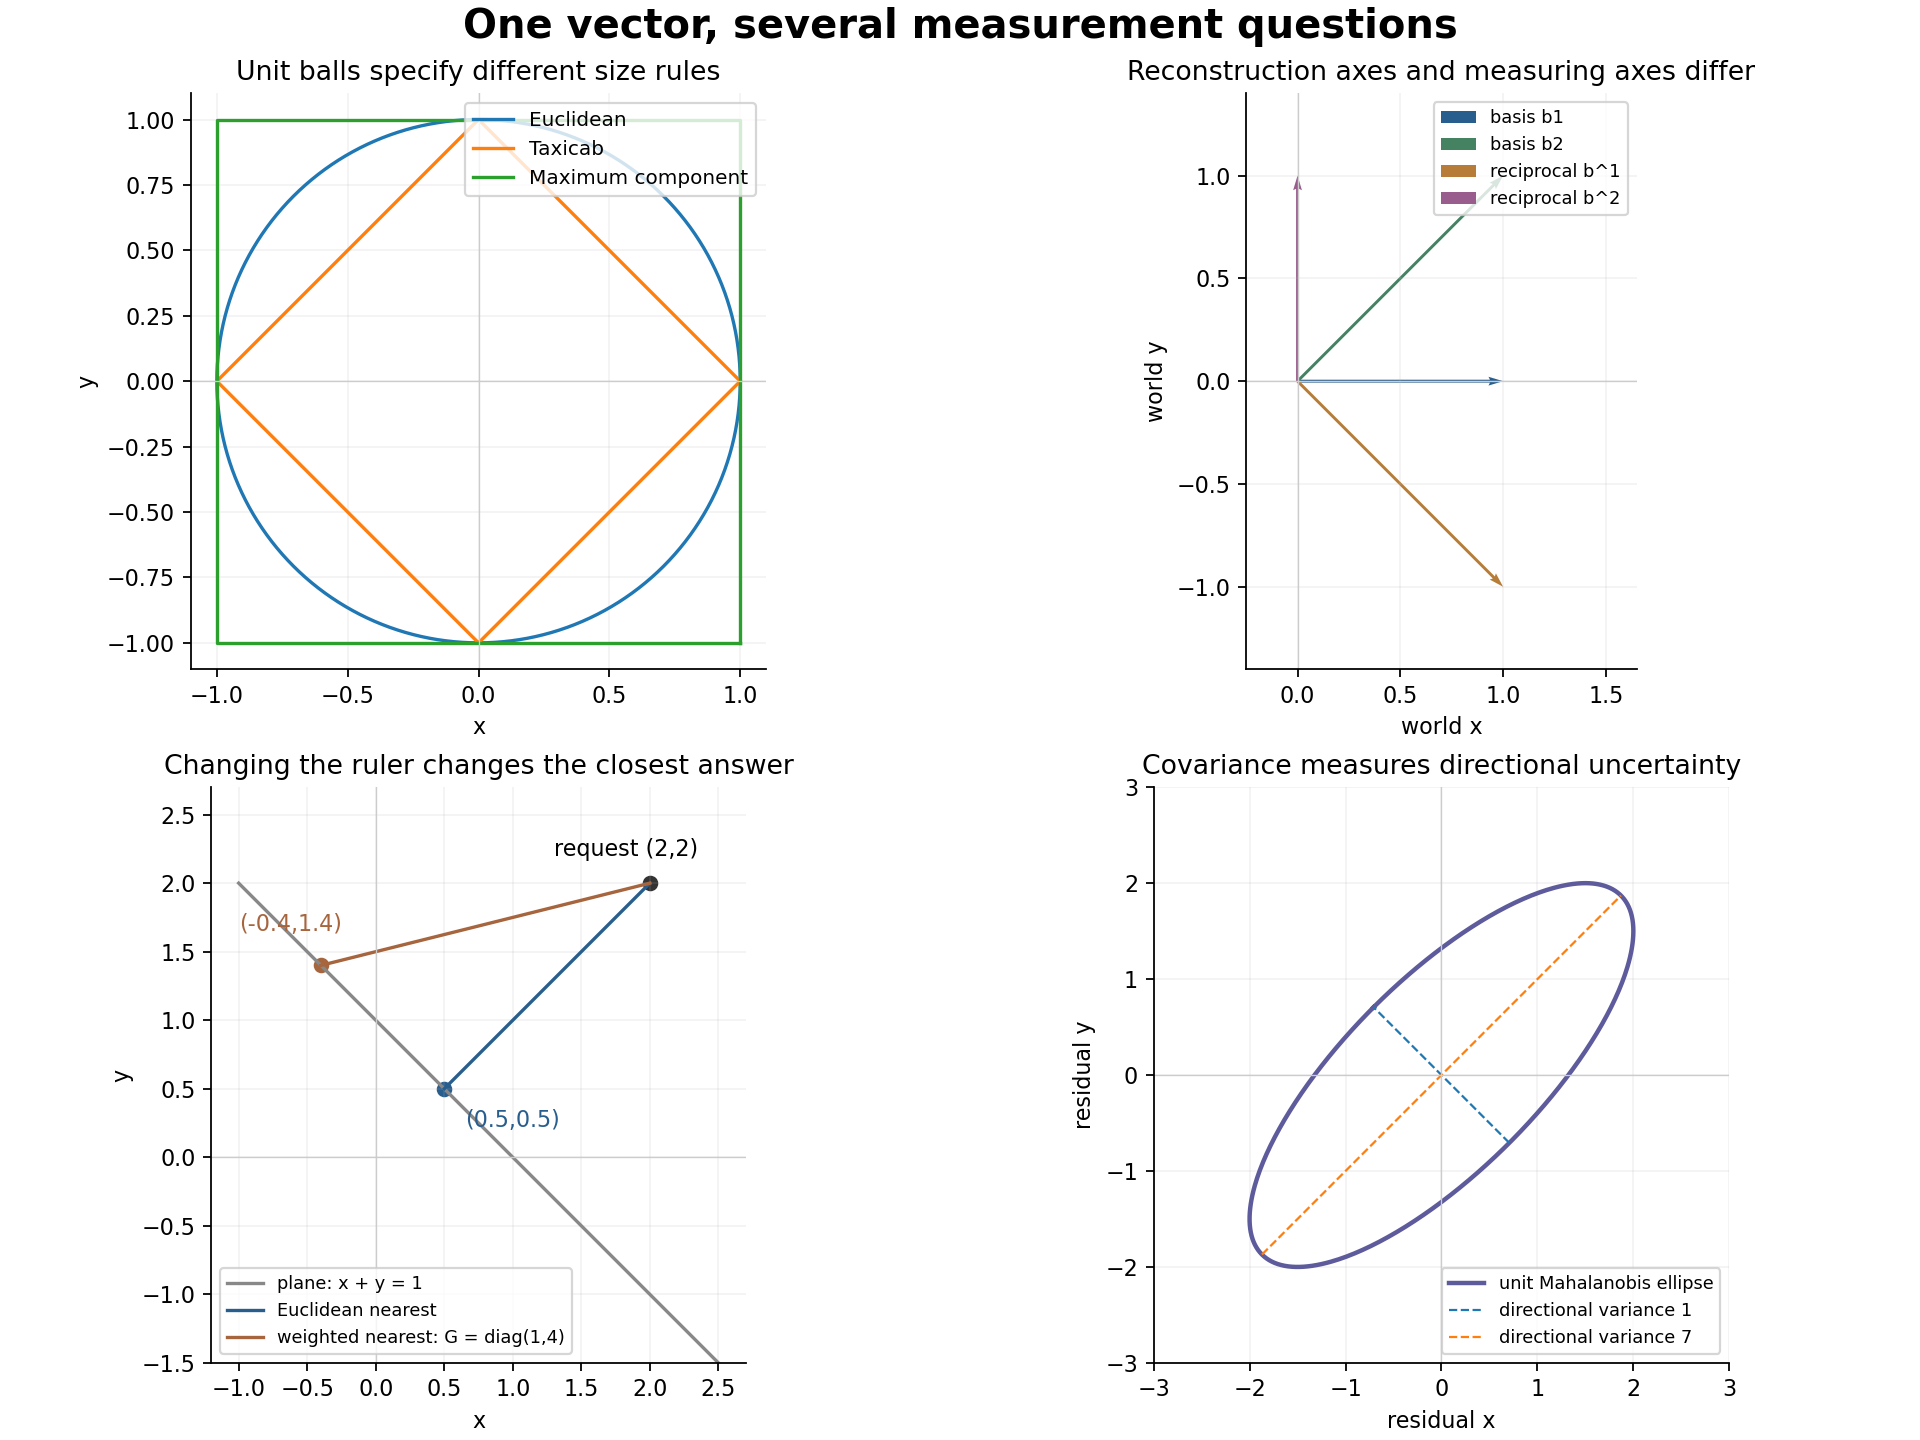
\includegraphics[keepaspectratio,alt={Visual Recall/Integrated Mathematics/metrics-and-measurements.png}]{Visual Recall/Integrated Mathematics/metrics-and-measurements.png}}
\caption{Visual Recall/Integrated Mathematics/metrics-and-measurements.png}
\end{figure}

{\def\LTcaptype{none} % do not increment counter
\begin{longtable}[]{@{}
  >{\raggedright\arraybackslash}p{(\linewidth - 4\tabcolsep) * \real{0.3333}}
  >{\raggedright\arraybackslash}p{(\linewidth - 4\tabcolsep) * \real{0.3333}}
  >{\raggedright\arraybackslash}p{(\linewidth - 4\tabcolsep) * \real{0.3333}}@{}}
\toprule\noalign{}
\begin{minipage}[b]{\linewidth}\raggedright
Prompt
\end{minipage} & \begin{minipage}[b]{\linewidth}\raggedright
Short answer
\end{minipage} & \begin{minipage}[b]{\linewidth}\raggedright
Explain immediately
\end{minipage} \\
\midrule\noalign{}
\endhead
\bottomrule\noalign{}
\endlastfoot
Why do dot measurements differ from coordinates? & A slanted reconstruction basis needs reciprocal measuring directions. & {[}{[}Continuous Notes/Computing Foundations - From Bits to C++ and Systems APIs\#Recover a component with the right measuring rule \\
Is every norm an ordinary dot-product length? & No.~The taxicab norm fails the parallelogram identity. & {[}{[}Continuous Notes/Computing Foundations - From Bits to C++ and Systems APIs\#Choose what a length is meant to measure \\
What does a dual norm measure? & Worst scalar response over an allowed vector-error ball. & {[}{[}Continuous Notes/Computing Foundations - From Bits to C++ and Systems APIs\#Bound a measurement using a dual norm \\
Is the Euclidean nearest point always the right constrained answer? & Only for that distance rule; a weighted ruler changes the correction direction. & {[}{[}Continuous Notes/Computing Foundations - From Bits to C++ and Systems APIs\#A rail, a wall, and a feasible region use the same nearest-point question \\
Differential or gradient? & A differential measures change; a metric turns it into a gradient vector. & {[}{[}Continuous Notes/Computing Foundations - From Bits to C++ and Systems APIs\#A derivative measures change; a gradient needs a ruler \\
Can a mesh boundary be a vector? & Yes: coefficients weight elements; boundary is linear. & {[}{[}Continuous Notes/Computing Foundations - From Bits to C++ and Systems APIs\#The same vector rules can describe a triangle's boundary \\
Are angle rates angular-velocity components? & Only in special configurations/conventions; instantaneous axes form a state-dependent map. & {[}{[}Continuous Notes/Computing Foundations - From Bits to C++ and Systems APIs\#Angle rates are not three components of angular velocity \\
Why is covariance directional? & A scalar measurement has variance \(a^{\mathsf T}\Sigma a\). & {[}{[}Continuous Notes/Computing Foundations - From Bits to C++ and Systems APIs\#Measure uncertainty along an actual direction \\
Is a unit uncertainty ellipse a 68\% region? & Not generally. The stated two-dimensional Gaussian unit ellipse contains about 39.35\%. & {[}{[}Continuous Notes/Computing Foundations - From Bits to C++ and Systems APIs\#Whiten residuals without pretending every ellipse has the same probability \\
How do vertex samples become a derivative? & Barycentric gradients reconstruct a constant field gradient per flat triangle. & {[}{[}Continuous Notes/Computing Foundations - From Bits to C++ and Systems APIs\#A triangle turns a differential into a concrete field calculation \\
\end{longtable}
}

The figure's four panels use the exact examples in those sections: norm balls, reciprocal directions, two constrained projections, and the covariance ellipse. Cover the answers and reconstruct one calculation from each panel. The book contains the assumptions and full derivations.
